\documentclass[oneside,11pt,a4paper,swedish]{scrbook}
\usepackage[utf8x]{inputenc}
\usepackage{babel}
\pagestyle{headings}
\setlength\parskip{\medskipamount}
\setlength\parindent{0pt}
\usepackage{graphicx}
\usepackage{ae}
\usepackage{aecompl}
\usepackage{amssymb}
\usepackage{amsmath}
\usepackage{comment}
\usepackage{nopageno}

\usepackage[T1]{fontenc}
%\usepackage{bookman}
\usepackage{multicol}
\usepackage{tikz}

\newcommand{\tavla}[1]{\reversemarginpar{ \rule[-10mm]{0.1mm}{#1cm}}}
\newcommand{\startex}[1]{\subsubsection{Exempel}\begin{quote}#1\end{quote}}
\newcommand{\startexn}[2]{\subsubsection{Exempel #1}\begin{quote}#2\end{quote}}

\newcommand{\ovning}[1]{\subparagraph{Övning: #1}}
\newcommand{\slutex}{\begin{flushright} \rule{1ex}{1ex} \end{flushright}}

\newcommand{\svarsrad}{\begin{flushright} \rule{14cm}{0.2mm} \end{flushright}}
\newcommand{\asm}[1]{\texttt{#1}}




\makeatother
\begin{document}

%%%%%%%%%%%%%%%%%%%%%%%%%%%%%%%%%%%%%%%%%%%%%%%%%%%%%%%%%%%
%linlog 1 decade START
%%%%%%%%%%%%%%%%%%%%%%%%%%%%%%%%%%%%%%%%%%%%%%%%%%%%%%%%%%
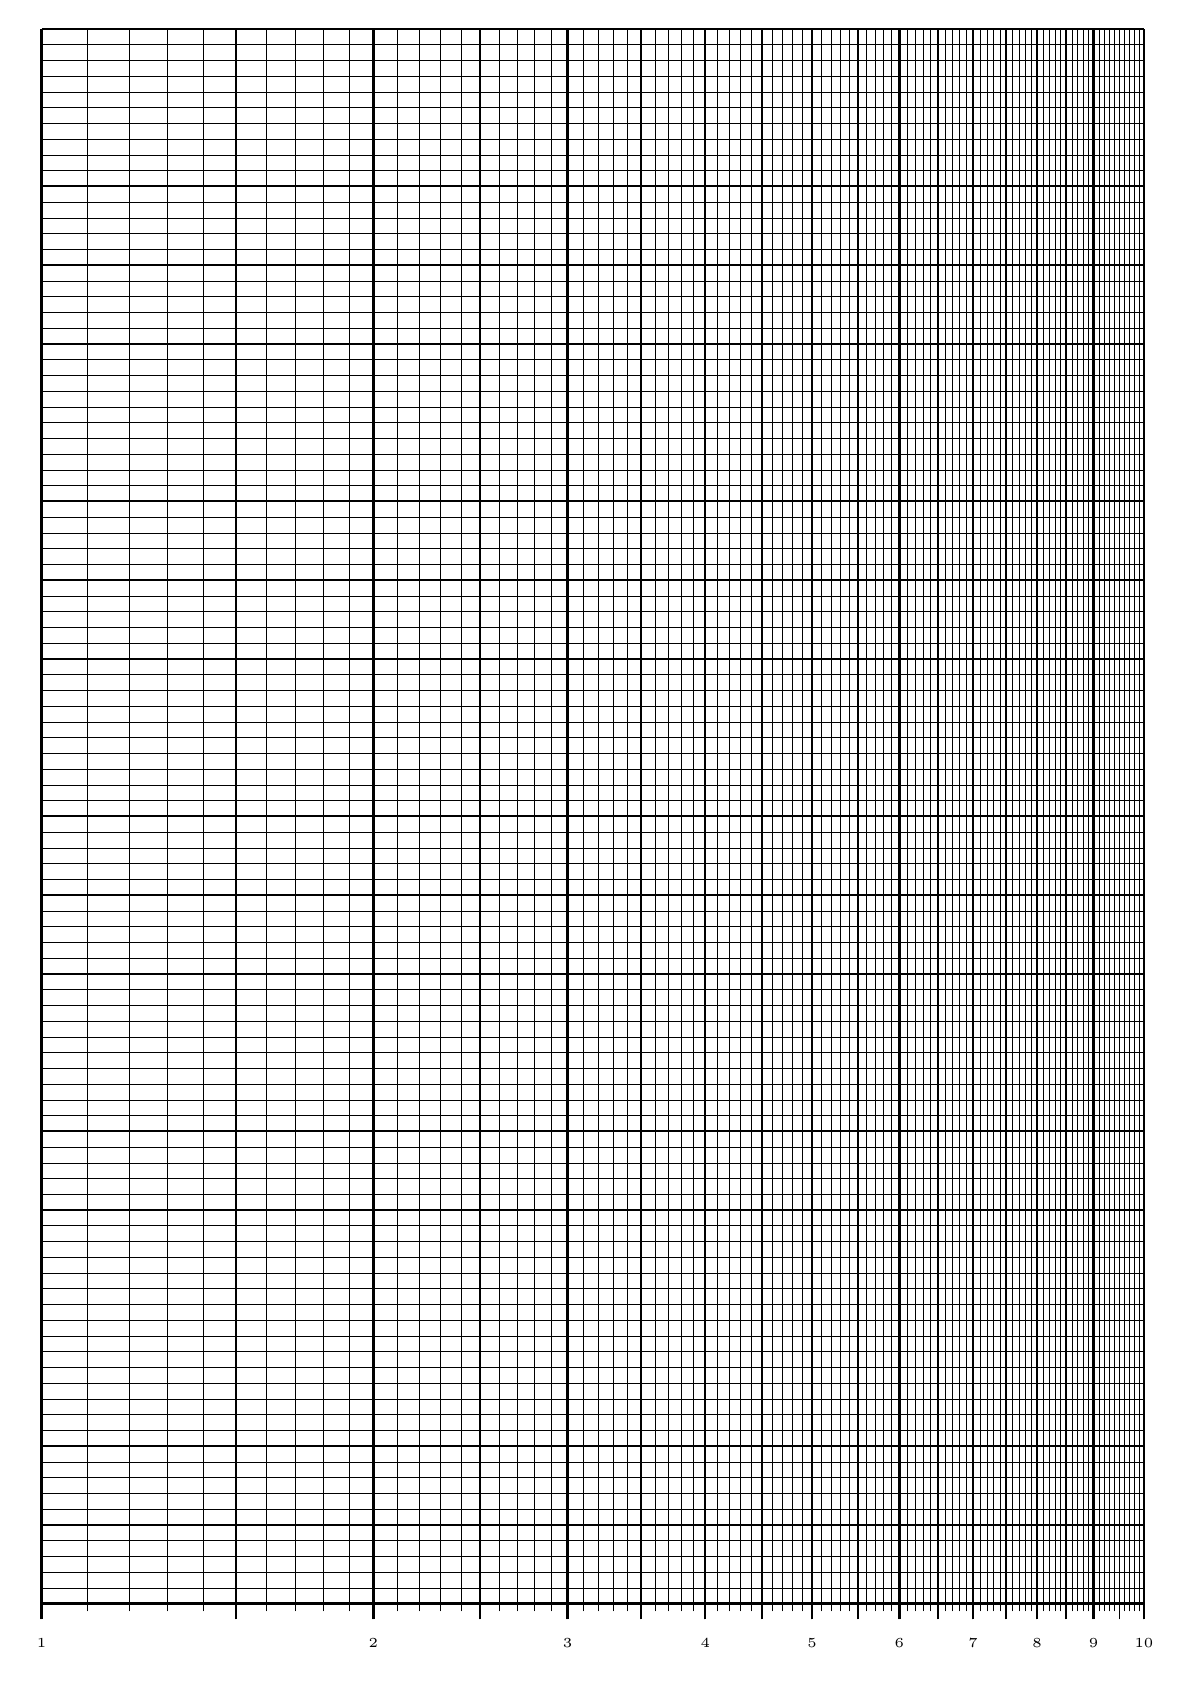
\begin{tikzpicture}[xscale=1,yscale=1] %[xscale=1.3,yscale=1.3]
\draw[thick] (0,0) --(14,0);
\foreach \x in {1,2,...,10} {
\node at (14/ln 10 *ln \x, -0.5) {\tiny{\pgfmathprintnumber[fixed,precision=1]{\x}}}; 
\draw[thick] (14/ln 10 *ln \x,-0.2) -- ( 14/ln 10 *ln \x ,20);
}
\foreach \x in {1,1.5,...,10} {
\draw[semithick] (14/ln 10 *ln \x,-0.2) -- ( 14/ln 10 *ln \x ,20);
}
\foreach \x in {1.0,1.1,...,10} {
\draw[ultra thin] (14/ln 10 *ln \x,-0.1) -- ( 14/ln 10 *ln \x ,20);
}
\foreach \x in {0.2,0.4,...,20} {
\draw[ultra thin] (0,\x) -- (14,\x);
}
\foreach \x in {1.0,2,...,20} {
\draw[semithick] (0,\x) -- (14,\x);
}
\end{tikzpicture}
%%%%%%%%%%%%%%%%%%%%%%%%%%%%%%%%%%%%%%%%%%%%%%%%%%%%%%%%%%%
%linlog 1 decade END
%%%%%%%%%%%%%%%%%%%%%%%%%%%%%%%%%%%%%%%%%%%%%%%%%%%%%%%%%%




%%%%%%%%%%%%%%%%%%%%%%%%%%%%%%%%%%%%%%%%%%%%%%%%%%%%%%%%%%%
%loglog 1 decade START
%%%%%%%%%%%%%%%%%%%%%%%%%%%%%%%%%%%%%%%%%%%%%%%%%%%%%%%%%%
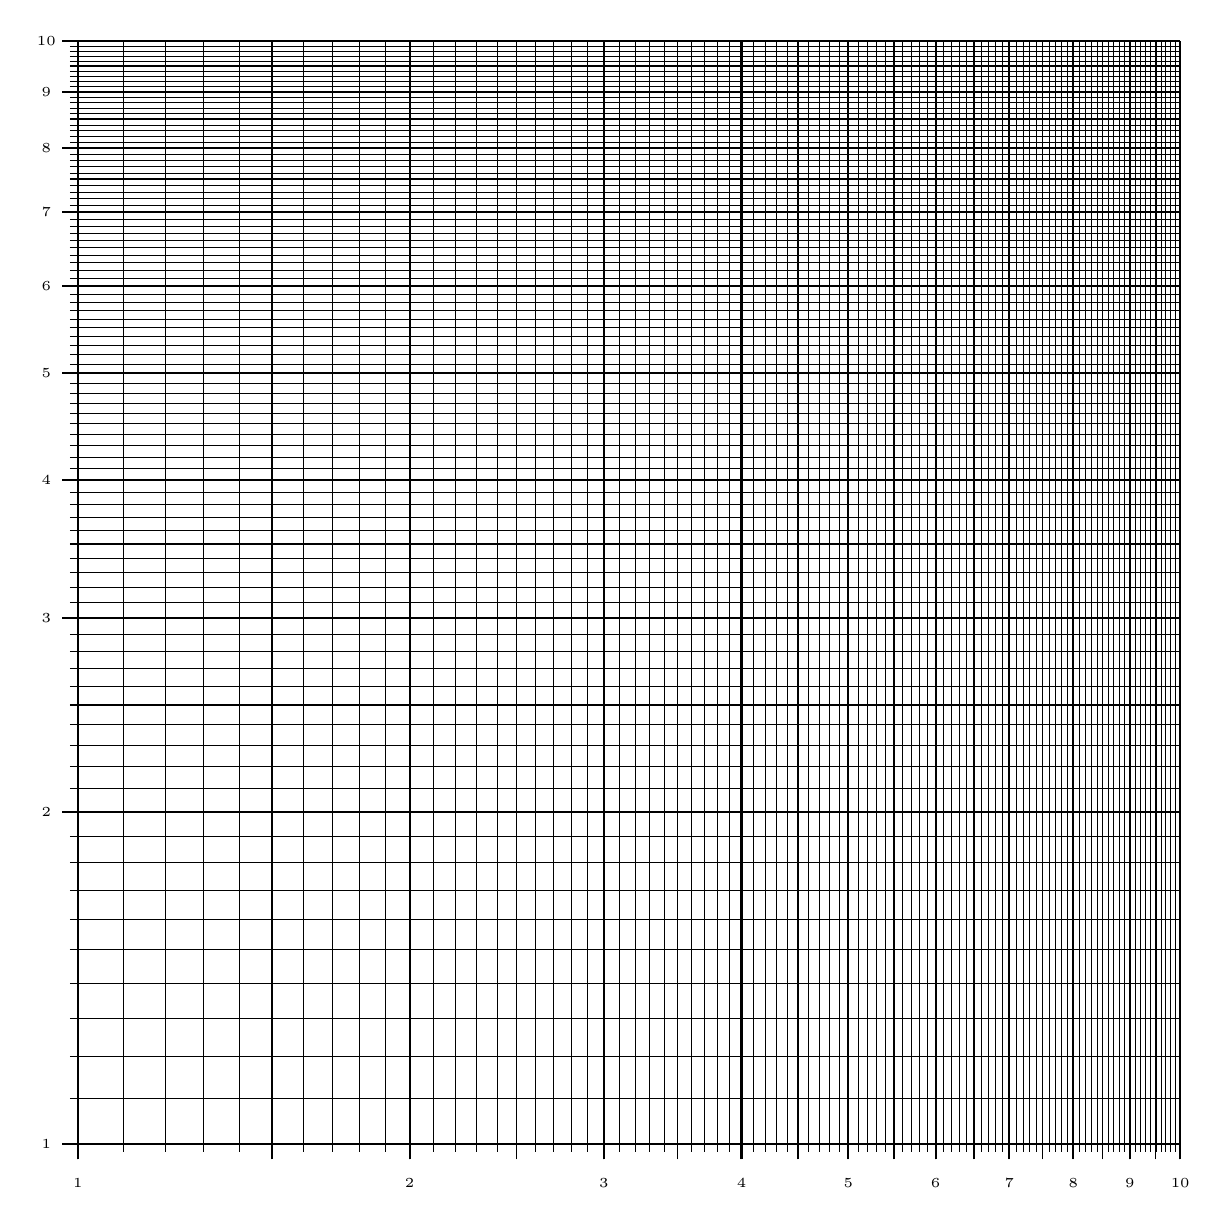
\begin{tikzpicture}[xscale=1,yscale=1] %[xscale=1.3,yscale=1.3]
\draw[ thick] (0,0) --(14,0);
\foreach \x in {1,2,...,10} {
\node at (14/ln 10 *ln \x, -0.5) {\tiny{\pgfmathprintnumber[fixed,precision=1]{\x}}}; 
\draw[thick] (14/ln 10 *ln \x,-0.2) -- ( 14/ln 10 *ln \x ,14);
}
\foreach \x in {1,1.5,...,10} {
\draw[semithick] (14/ln 10 *ln \x,-0.2) -- ( 14/ln 10 *ln \x ,14);
}
\foreach \x in {1.0,1.1,...,10} {
\draw[ultra thin] (14/ln 10 *ln \x,-0.1) -- ( 14/ln 10 *ln \x ,14);
}
\foreach \x in {1,2,...,10} {
\node at (-0.4, 14/ln 10 *ln \x) {\tiny{\pgfmathprintnumber[fixed,precision=1]{\x}}}; 
\draw[thick] (-0.2 ,14/ln 10 *ln \x) -- ( 14 ,14/ln 10 *ln \x);
}
\foreach \x in {1,1.5,...,10} {
\draw[semithick] (-0.1, 14/ln 10 *ln \x) -- ( 14, 14/ln 10 *ln \x);
}
\foreach \x in {1.0,1.1,...,10} {
\draw[ultra thin] (-0.1, 14/ln 10 *ln \x) -- ( 14, 14/ln 10 *ln \x);
}

\end{tikzpicture}
%%%%%%%%%%%%%%%%%%%%%%%%%%%%%%%%%%%%%%%%%%%%%%%%%%%%%%%%%%%
%loglog 1 decade END
%%%%%%%%%%%%%%%%%%%%%%%%%%%%%%%%%%%%%%%%%%%%%%%%%%%%%%%%%%




%%%%%%%%%%%%%%%%%%%%%%%%%%%%%%%%%%%%%%%%%%%%%%%%%%%%%%%%%%%
%loglog 3 decade START
%%%%%%%%%%%%%%%%%%%%%%%%%%%%%%%%%%%%%%%%%%%%%%%%%%%%%%%%%%

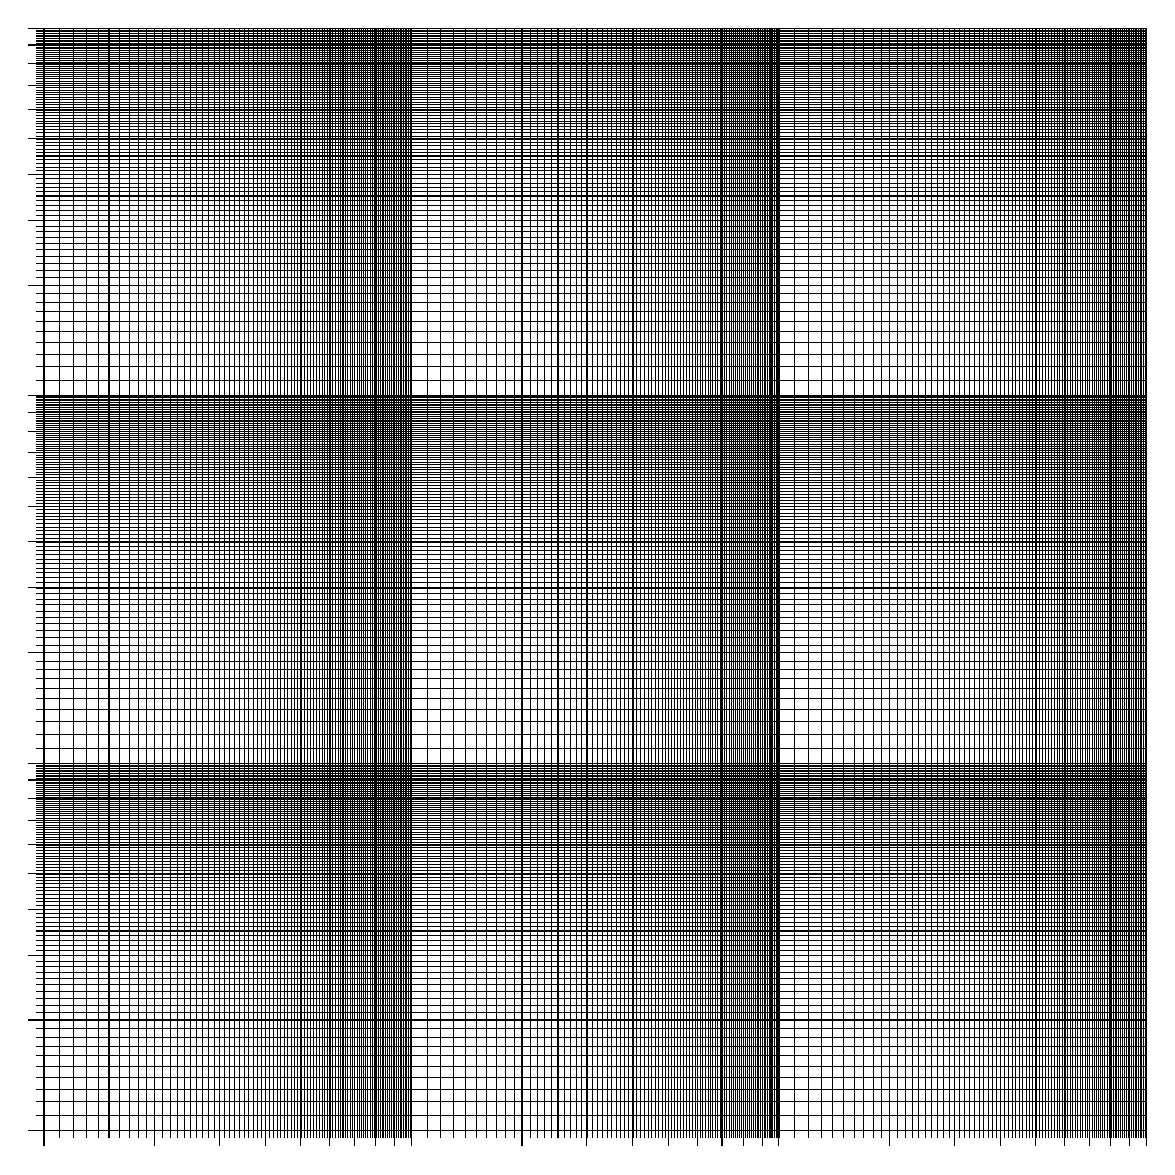
\begin{tikzpicture}[xscale=1,yscale=1] %[xscale=1.3,yscale=1.3]
\draw[ thin] (0,0) --(14,0);
% xaxis
% 1st decade
\foreach \x in {1,2,...,10} {
%\node at (14/2/ln 10 *ln \x, -0.5) {\pgfmathprintnumber[fixed,precision=1]{\x}}; 
\draw[thin] (14/3/ln 10 *ln \x,-0.2) -- ( 14/3/ln 10 *ln \x ,14);
}
\foreach \x in {1,1.5,...,10} {
\draw[very thin] (14/3/ln 10 *ln \x,-0.1) -- ( 14/3/ln 10 *ln \x ,14);
}
\foreach \x in {1.0,1.1,...,10} {
\draw[ultra thin] ( 14/3/ln 10 *ln \x, -0.1) -- ( 14/3/ln 10 *ln \x, 14);
}

% xaxis 
% 2nd decade
\foreach \x in {1,2,...,10} {
%\node at (14/2/ln 10 *ln \x+14/2, -0.5) {\pgfmathprintnumber[fixed,precision=1]{\x}}; 
\draw[thin] (14/3/ln 10 *ln \x+14/3,-0.2) -- ( 14/3/ln 10 *ln \x +14/3,14);
}
\foreach \x in {1,1.5,...,10} {
\draw[very thin] (14/3/ln 10 *ln \x+14/3,-0.1) -- ( 14/3/ln 10 *ln \x +14/3,14);
}
\foreach \x in {1.0,1.1,...,10} {
\draw[ultra thin] ( 14/3/ln 10 *ln \x+14/3, -0.1) -- ( 14/3/ln 10 *ln \x+14/3, 14);
}

% xaxis 
% 3rd decade
\foreach \x in {1,2,...,10} {
%\node at (14/2/ln 10 *ln \x+14/2, -0.5) {\pgfmathprintnumber[fixed,precision=1]{\x}}; 
\draw[thin] (14/3/ln 10 *ln \x+14/3+14/3,-0.2) -- ( 14/3/ln 10 *ln \x +14/3+14/3,14);
}
\foreach \x in {1,1.5,...,10} {
\draw[ very thin] (14/3/ln 10 *ln \x+14/3+14/3,-0.1) -- ( 14/3/ln 10 *ln \x +14/3+14/3,14);
}
\foreach \x in {1.0,1.1,...,10} {
\draw[ultra thin] ( 14/3/ln 10 *ln \x+14/3+14/3, -0.1) -- ( 14/3/ln 10 *ln \x+14/3+14/3, 14);
}

%\foreach \x in {1.0,1.1,...,10} {
%\draw[ultra thin] (14/ln 10 *ln \x,-0.1) -- ( 14/ln 10 *ln \x ,14);
%}
% yaxis
% 1st decade
\foreach \x in {1,2,...,10} {
%\node at (-0.4, 14/2/ln 10 *ln \x) {\tiny{\pgfmathprintnumber[fixed,precision=1]{\x}}}; 
\draw[thin] (-0.2 ,14/3/ln 10 *ln \x) -- ( 14 ,14/3/ln 10 *ln \x);
}
\foreach \x in {1,1.5,...,10} {
\draw[ very thin] (-0.1, 14/3/ln 10 *ln \x) -- ( 14, 14/3/ln 10 *ln \x);
}
\foreach \x in {1.0,1.1,...,10} {
\draw[ultra thin] (-0.1, 14/3/ln 10 *ln \x) -- ( 14, 14/3/ln 10 *ln \x);
}

% yaxis
% 2nd decade
\foreach \x in {2,3,...,10} {
%\node at (-0.4, 14/2/ln 10 *ln \x+14/2) {\tiny{\pgfmathprintnumber[fixed,precision=1]{\x}}}; 
\draw[thin] (-0.2 ,14/3/ln 10 *ln \x+14/3) -- ( 14 ,14/3/ln 10 *ln \x+14/3);
}
\foreach \x in {1,1.5,...,10} {
\draw[very thin] (-0.1, 14/3/ln 10 *ln \x+14/3) -- ( 14, 14/3/ln 10 *ln \x+14/3);
}
\foreach \x in {1.0,1.1,...,10} {
\draw[ultra thin] (-0.1, 14/3/ln 10 *ln \x+14/3) -- ( 14, 14/3/ln 10 *ln \x+14/3);
}
% yaxis
% 3rd decade
\foreach \x in {2,3,...,10} {
%\node at (-0.4, 14/3/ln 10 *ln \x+14/2) {\tiny{\pgfmathprintnumber[fixed,precision=1]{\x}}}; 
\draw[thin] (-0.2 ,14/3/ln 10 *ln \x+14/3+14/3) -- ( 14 ,14/3/ln 10 *ln \x+14/3+14/3);
}
\foreach \x in {1,1.5,...,10} {
\draw[very thin] (-0.1, 14/3/ln 10 *ln \x+14/3+14/3) -- ( 14, 14/3/ln 10 *ln \x+14/3+14/3);
}
\foreach \x in {1.0,1.1,...,10} {
\draw[ultra thin] (-0.1, 14/3/ln 10 *ln \x+14/3+14/3) -- ( 14, 14/3/ln 10 *ln \x+14/3+14/3);
}


\end{tikzpicture}
%%%%%%%%%%%%%%%%%%%%%%%%%%%%%%%%%%%%%%%%%%%%%%%%%%%%%%%%%%%
%loglog 3 decade END
%%%%%%%%%%%%%%%%%%%%%%%%%%%%%%%%%%%%%%%%%%%%%%%%%%%%%%%%%%






%%%%%%%%%%%%%%%%%%%%%%%%%%%%%%%%%%%%%%%%%%%%%%%%%%%%%%%%%%%
%linlog 3 decade START
%%%%%%%%%%%%%%%%%%%%%%%%%%%%%%%%%%%%%%%%%%%%%%%%%%%%%%%%%%
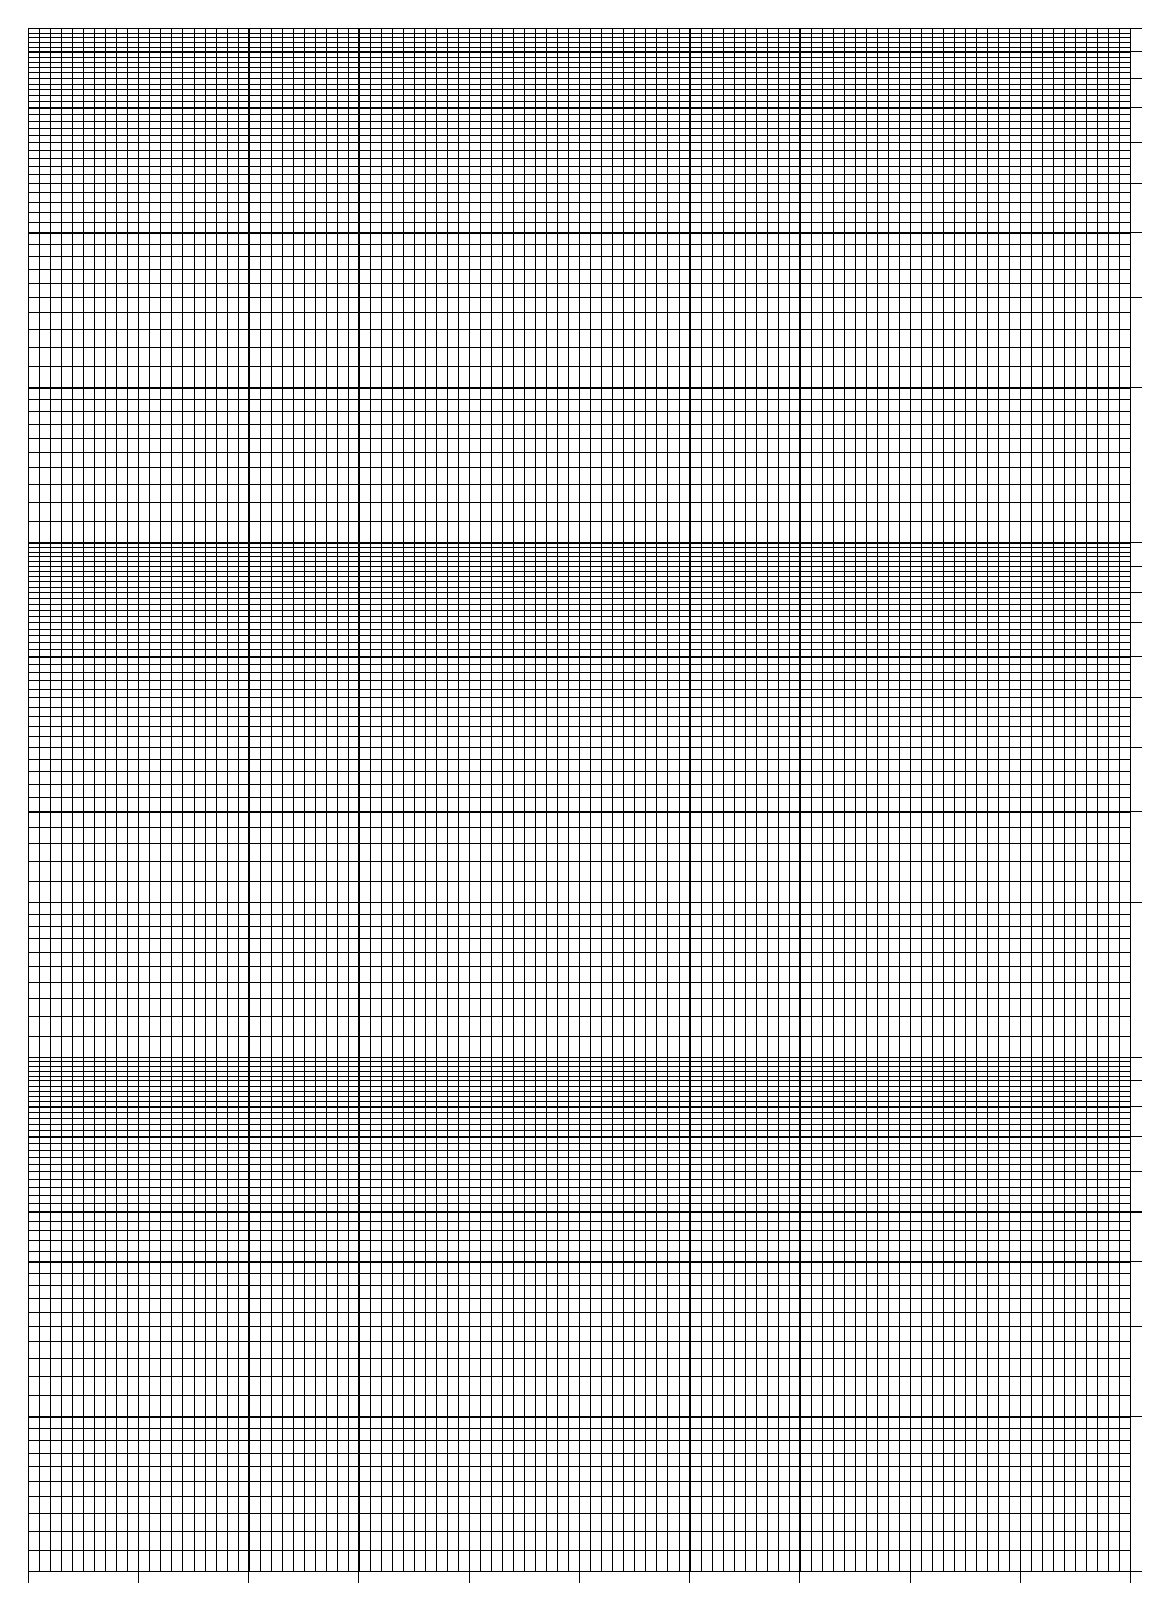
\begin{tikzpicture}[rotate=90,scale=1.4] %[xscale=1.3,yscale=1.3]
\draw[thin] (-0.1,0) --(14,0);

\foreach \x in {1,2,...,10} {
%\node at (7/ln 10 *ln \x, -0.5) {\pgfmathprintnumber[fixed,precision=1]{\x}}; 
\draw[thin] (14/3/ln 10 *ln \x,-0.1) -- ( 14/3/ln 10 *ln \x ,10);
}
\foreach \x in {1,1.1,...,2} {
\draw[ultra thin] (14/3/ln 10 *ln \x,0) -- ( 14/3/ln 10 *ln \x ,10);
}
\foreach \x in {2,2.2,...,10} {
\draw[ultra thin] (14/3/ln 10 *ln \x,0) -- ( 14/3/ln 10 *ln \x ,10);
}

\foreach \x in {1,2,...,10} {
\draw[thin] (14/3/ln 10 *ln \x+14/3,-0.1) -- ( 14/3/ln 10 *ln \x +14/3,10);
}
\foreach \x in {1,1.1,...,2} {
\draw[ultra thin] (14/3/ln 10 *ln \x+14/3,0) -- ( 14/3/ln 10 *ln \x+14/3 ,10);
}
\foreach \x in {2,2.2,...,10} {
\draw[ultra thin] (14/3/ln 10 *ln \x+14/3,0) -- ( 14/3/ln 10 *ln \x+14/3 ,10);
}

\foreach \x in {1,2,...,10} {
\draw[thin] (14/3/ln 10 *ln \x+14/3 +14/3,-0.1) -- ( 14/3/ln 10 *ln \x +14/3+14/3,10);
}
\foreach \x in {1,1.1,...,2} {
\draw[ultra thin] (14/3/ln 10 *ln \x+14/3+14/3,0) -- ( 14/3/ln 10 *ln \x +14/3+14/3,10);
}
\foreach \x in {2,2.2,...,10} {
\draw[ultra thin] (14/3/ln 10 *ln \x+14/3+14/3,0) -- ( 14/3/ln 10 *ln \x +14/3+14/3,10);
}


\foreach \x in {0.1,0.2,...,10} {
\draw[ultra thin] (0,\x) -- (14,\x);
}
\foreach \x in {1.0,2,...,10} {
\draw[thin] (-0.1,\x) -- (14,\x);
}
\end{tikzpicture}

%%%%%%%%%%%%%%%%%%%%%%%%%%%%%%%%%%%%%%%%%%%%%%%%%%%%%%%%%%%
%Linlog 3 decade END
%%%%%%%%%%%%%%%%%%%%%%%%%%%%%%%%%%%%%%%%%%%%%%%%%%%%%%%%%%


\end{document}